% report.tex -- A3: Benchmarking Approximate Nearest Neighbour Search (CS4.406 IRE)
% FIRST DRAFT written by Claude (AI-generated) for Samarth to check, rewrite and shorten.
% Every number comes from a file in ../results/ (or config.py / hypothesis.md); each paragraph
% ends with a "% SOURCE:" comment naming the file(s). Tables are \input from ../results/tables/
% (regenerated by experiments/make_tables.py) and figures from ../results/figures/.
\documentclass[11pt]{article}
\usepackage[margin=2cm]{geometry}
\usepackage[T1]{fontenc}
\usepackage{lmodern}
\usepackage{graphicx}
\usepackage{booktabs}
\usepackage{adjustbox}
\usepackage{array}
\usepackage{amsmath}
\usepackage[section]{placeins}
\usepackage{caption}
\usepackage[hidelinks]{hyperref}
\captionsetup{font=small}
\graphicspath{{../results/figures/}}
\setlength{\parskip}{0.3em}

\title{Benchmarking Approximate Nearest Neighbour Search}
\author{Samarth (2024101020)\\CS4.406 Information Retrieval \& Extraction, Assignment 3}
\date{October 2026}

\begin{document}
\maketitle

%======================================================================
\section{Setup}

\textbf{Machine and libraries.} All numbers come from one laptop: an Intel Core i7-13700H with
14 physical and 20 logical cores and 15.75\,GB of RAM, running Windows
(\texttt{Windows-10-10.0.26200}). The software is Python 3.11.17, FAISS 1.14.3 (faiss-cpu, conda-forge), numpy 2.4.6,
h5py 3.16.0, pandas 3.1.0 and matplotlib 3.11.2, with OpenBLAS 0.3.34 (pthreads) as the BLAS
library. hnswlib was not used; HNSW is FAISS's \texttt{IndexHNSWFlat}. Index building uses all 20
logical CPUs.
% SOURCE: results/env.json

\textbf{Data.} SIFT has 1,000,000 base vectors in 128 dimensions; GloVe-100 has 1,183,514 in 100
dimensions; each has 10,000 queries. GloVe base vectors and queries are L2-normalised (no
zero-norm vectors were found), so Euclidean order equals angular order and squared L2 is used
everywhere. The first 5,000 queries are for tuning and the last 5,000 for reporting.
% SOURCE: results/part1_agreement.json (n_base, metric_note), config.py (TUNE, TEST)

\textbf{Recall.} Recall@10 is tie-aware. Let $d_{10}$ be the true squared distance of the
10th exact neighbour. A returned id counts as correct if its true distance is at most
$d_{10}(1+\epsilon)+\epsilon_{\mathrm{abs}}$, with $\epsilon=10^{-5}$ and
$\epsilon_{\mathrm{abs}}=10^{-6}$. Duplicate and $-1$ ids are ignored, and recall@10 is
$\min(\#\text{correct},10)/10$ averaged over queries. True distances are recomputed from the
vectors in float64, never taken from the index (PQ distances are approximate). Ground truth is
our own exact top-100 from FAISS \texttt{IndexFlatL2}. The function has 11 unit tests.
% SOURCE: annbench/metrics.py, config.py (RECALL_REL_EPS, RECALL_ABS_EPS), tests/test_recall.py

\textbf{Timing protocol.}
\begin{itemize}
\item Speed is queries per second (QPS), one query per call, on a single thread (one FAISS
  OpenMP thread and one BLAS thread), with the process pinned to logical CPU 2, a performance
  core.
\item Each measurement is one untimed warm-up pass plus 3 timed passes, and we report the median.
\item Tuning uses the first 2,000 tune queries. A sweep stops once test recall is at least
  0.999 for two points in a row.
\item An operating point at a target recall is the fastest config whose \emph{tune} recall
  reaches the target. We then report that config's \emph{test} recall and QPS as measured.
\item Before each sweep a fixed exact search (200 queries on 20,000 vectors) is timed as a
  ``canary'' that tracks machine-state drift.
\end{itemize}
% SOURCE: config.py (PIN_CPU, REPEATS, WARMUP, TUNE_N, EARLY_STOP_*, CANARY_*), annbench/timing.py

%======================================================================
\section{Part 1: Exact baseline}

\begin{table}[t]
\centering
\small
\begin{adjustbox}{max width=\linewidth}
\begin{tabular}{lrrrrrrr}
\toprule
Dataset & n & Exact top-10 set match & Tie-aware recall vs file & Single-query QPS & Batch QPS (1 thread) & Batch QPS (all threads) & Batch / single (1 thread) \\
\midrule
sift & 1,000,000 & 0.9935 (10,000 q) & 1.0000 & 30.8 (32.5 ms) & 342 & 761 (20 thr) & 11.1$\times$ \\
glove & 1,183,514 & 1.0000 (10,000 q) & 1.0000 & 34.4 (29.1 ms) & 348 & 383 (20 thr) & 10.1$\times$ \\
\bottomrule
\end{tabular}
\end{adjustbox}
\caption{Exact search (IndexFlatL2). Agreement with the neighbours stored in the data file (full-size data). Single-query timing: first 1,000 test queries, 1 thread, pinned; batch: 5,000 test queries in one call. Median of 3 runs.}
\label{tab:part1}
\end{table}


\textbf{Agreement.} Our exact top-10 matches the file's neighbour sets for 99.35\% of SIFT
queries and for every GloVe query. All 65 SIFT mismatches are ties: our point and the file's
point have the same distance to the query as the 10th neighbour (for example 40,644.0 in
squared distance). SIFT's integer coordinates make exact ties common. With ties allowed,
recall of our results against the file is 1.0000 on both datasets, and in the other direction
too. The file's distances also match ours to a relative difference of $1.2\times10^{-7}$ on
SIFT and $1.6\times10^{-7}$ on GloVe (after converting GloVe's angular distance to squared L2).
% SOURCE: results/part1_agreement.json, results/tables/part1.tex

\textbf{Single query vs batch.} One query at a time, exact search runs at 30.8\,QPS on SIFT
(32.5\,ms per query) and 34.4\,QPS on GloVe. Searching all 5,000 test queries in one call on the
same single thread runs at 342 and 348\,QPS, which is 11.1$\times$ and 10.1$\times$ faster.
\begin{itemize}
\item \emph{Batch:} FAISS turns a batch into one matrix--matrix product (BLAS GEMM). Each base
  vector is loaded from memory once and reused for many queries while it sits in cache, and the
  blocked kernel keeps the SIMD units busy.
\item \emph{One at a time:} each query is a matrix--vector product. It streams every base vector (512 bytes each on SIFT) from RAM again, so it is limited by
  memory bandwidth, not arithmetic, and it also pays a per-call overhead.
\end{itemize}
With all 20 threads the batch reaches 761\,QPS on SIFT, but only 383\,QPS on GloVe; we did not
find out why GloVe scales so poorly.
% SOURCE: results/tables/part1.tex, results/part1_notes.md, results/tables/part2_cost.tex (512 B/vector)

%======================================================================
\section{Part 2: Benchmark of HNSW, IVF-Flat and IVF-PQ}

\textbf{What was run.}
\begin{itemize}
\item \emph{HNSW:} $M\in\{16,32,48\}$ with efConstruction 200, sweeping efSearch from 10 to 512.
\item \emph{IVF-Flat:} nlist $\in\{1024,4096,8192\}$, sweeping nprobe from 1 to 512.
\item \emph{IVF-PQ:} nlist $\in\{1024,4096\}$ with 8-bit codes, $m\in\{16,32,64\}$ on SIFT and
  $\{20,25,50\}$ on GloVe, sweeping nprobe.
\end{itemize}
For GloVe, two sweeps never reached 0.95 (HNSW $M{=}16$ and IVF-Flat nlist 8192), so they were
extended to efSearch 1024 and nprobe 1024. Figure~\ref{fig:part2} shows the best trade-off curve
for each index with the exact baseline; Tables~\ref{tab:part2_qps} and~\ref{tab:part2_cost} give
QPS, build cost and memory at the operating points.
% SOURCE: config.py (GRIDS, SWEEP_EXTEND)

\begin{figure}[t]
\centering
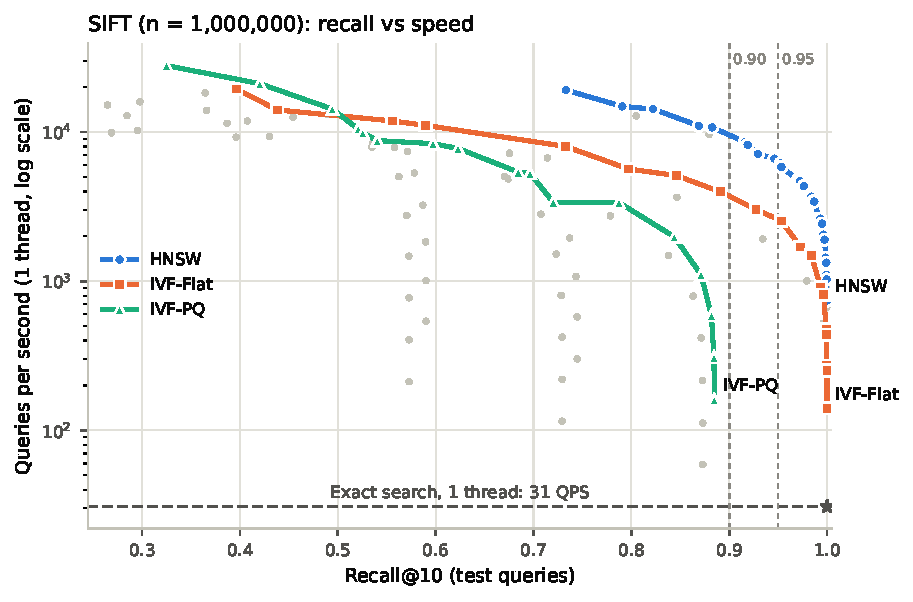
\includegraphics[width=0.495\linewidth]{part2_sift.pdf}\hfill
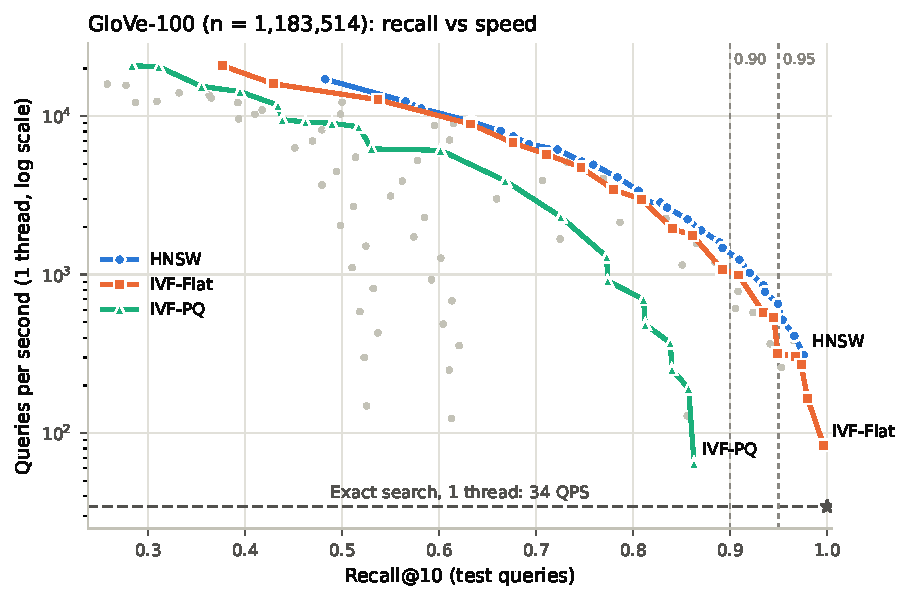
\includegraphics[width=0.495\linewidth]{part2_glove.pdf}
\caption{Recall@10 (test queries) against single-thread QPS (log scale). Lines: Pareto frontier
of each index over all build settings; grey dots: other configs; dashed line: exact search.}
\label{fig:part2}
\end{figure}

\begin{table}[t]
\centering
\small
\begin{adjustbox}{max width=\linewidth}
\begin{tabular}{llrrp{2.6cm}rrp{2.6cm}r}
\toprule
Dataset & Index & QPS @0.90 & Recall & Config @0.90 & QPS @0.95 & Recall & Config @0.95 & Speed-up vs exact (0.90 / 0.95) \\
\midrule
sift & HNSW & 8,581 & 0.916 & M=16, efSearch=32 & 4,775 & 0.970 & M=16, efSearch=64 & 279$\times$ / 155$\times$ \\
sift & IVF-Flat & 3,030 & 0.927 & nlist=4096, nprobe=32 & 1,697 & 0.973 & nlist=4096, nprobe=64 & 98$\times$ / 55$\times$ \\
sift & IVF-PQ & not reached & max 0.885 & nlist=4096, m=64, nprobe=512 & not reached & max 0.885 & nlist=4096, m=64, nprobe=512 & - / - \\
glove & HNSW & 1,241 & 0.910 & M=48, efSearch=128 & 518 & 0.954 & M=32, efSearch=384 & 36$\times$ / 15$\times$ \\
glove & IVF-Flat & 995 & 0.909 & nlist=8192, nprobe=256 & 303 & 0.967 & nlist=4096, nprobe=512 & 29$\times$ / 9$\times$ \\
glove & IVF-PQ & not reached & max 0.863 & nlist=1024, m=50, nprobe=512 & not reached & max 0.863 & nlist=1024, m=50, nprobe=512 & - / - \\
\bottomrule
\end{tabular}
\end{adjustbox}
\caption{Single-thread, one-query-at-a-time QPS on the test queries (median of 3 runs) at recall@10 0.90 and 0.95. Configs are chosen on the tune queries (recall $\geq$ target); test recall is reported as measured and may fall slightly below the target. 'not reached': no config reached the target on the tune queries; the highest-recall config is shown with its test recall.}
\label{tab:part2_qps}
\end{table}

\begin{table}[t]
\centering
\small
\begin{tabular}{lllrrrrr}
\toprule
Dataset & Index & Config @0.95 & Build time s (threads) & Train s & Size MB & Bytes/vector & Raw float32 bytes/vector \\
\midrule
sift & HNSW & M=16, efSearch=64 & 60.8 (20 thr) & 0.0 & 625.9 & 656.3 & 512 \\
sift & IVF-Flat & nlist=4096, nprobe=64 & 18.9 (20 thr) & 13.5 & 497.9 & 522.1 & 512 \\
sift & IVF-PQ & not reached (max recall 0.885): nlist=4096, m=64, nprobe=512 & 62.3 (20 thr) & 51.7 & 70.8 & 74.3 & 512 \\
glove & HNSW & M=32, efSearch=384 & 149.2 (20 thr) & 0.0 & 758.6 & 672.2 & 400 \\
glove & IVF-Flat & nlist=4096, nprobe=512 & 18.1 (20 thr) & 12.4 & 462.1 & 409.4 & 400 \\
glove & IVF-PQ & not reached (max recall 0.863): nlist=1024, m=50, nprobe=512 & 35.4 (20 thr) & 29.2 & 66.0 & 58.4 & 400 \\
\bottomrule
\end{tabular}
\caption{Build cost and memory of the config chosen at recall 0.95 (or the highest-recall config if 0.95 is not reached). Size = serialised index. Configs are chosen on the tune queries (recall $\geq$ target); test recall is reported as measured and may fall slightly below the target.}
\label{tab:part2_cost}
\end{table}


\textbf{Results.} At recall 0.95, HNSW is the fastest index on both datasets.
\begin{itemize}
\item \emph{SIFT:} HNSW runs at 4,775\,QPS (155$\times$ exact, $M{=}16$, efSearch 64) and
  IVF-Flat at 1,697\,QPS (55$\times$).
\item \emph{GloVe:} HNSW runs at 518\,QPS (15$\times$, $M{=}32$, efSearch 384) and IVF-Flat at
  303\,QPS (9$\times$).
\end{itemize}
% SOURCE: results/tables/part2_qps.tex

\textbf{Why IVF-PQ fails.} IVF-PQ never reaches 0.90 on either dataset. Its best test recall is
0.885 on SIFT and 0.863 on GloVe, at the largest $m$ and nprobe 512. PQ compares queries with
quantised codes, not the vectors themselves. The quantisation error does not depend on nprobe,
so whenever the true 10th and 11th neighbours are closer together than that error they get
mis-ordered. Searching more lists cannot fix this; only re-ranking with exact distances can
(Part 3).
% SOURCE: results/tables/part2_qps.tex, results/part2_notes.md

%======================================================================
\section{Part 3: Compression on SIFT}

\textbf{Experiment.} We fix nlist $=4096$ and 8-bit codes and vary the number of PQ sub-vectors
$m\in\{8,16,32,64\}$. For each $m$ we sweep nprobe for two variants: plain IVF-PQ, and the
\emph{same} trained index wrapped in \texttt{IndexRefineFlat} (k\_factor 10). The wrapper
re-ranks the top 100 PQ candidates with exact distances, so re-ranking is the only difference.
The hypothesis was committed before the run.
% SOURCE: config.py (PART3), hypothesis.md

\begin{figure}[t]
\centering
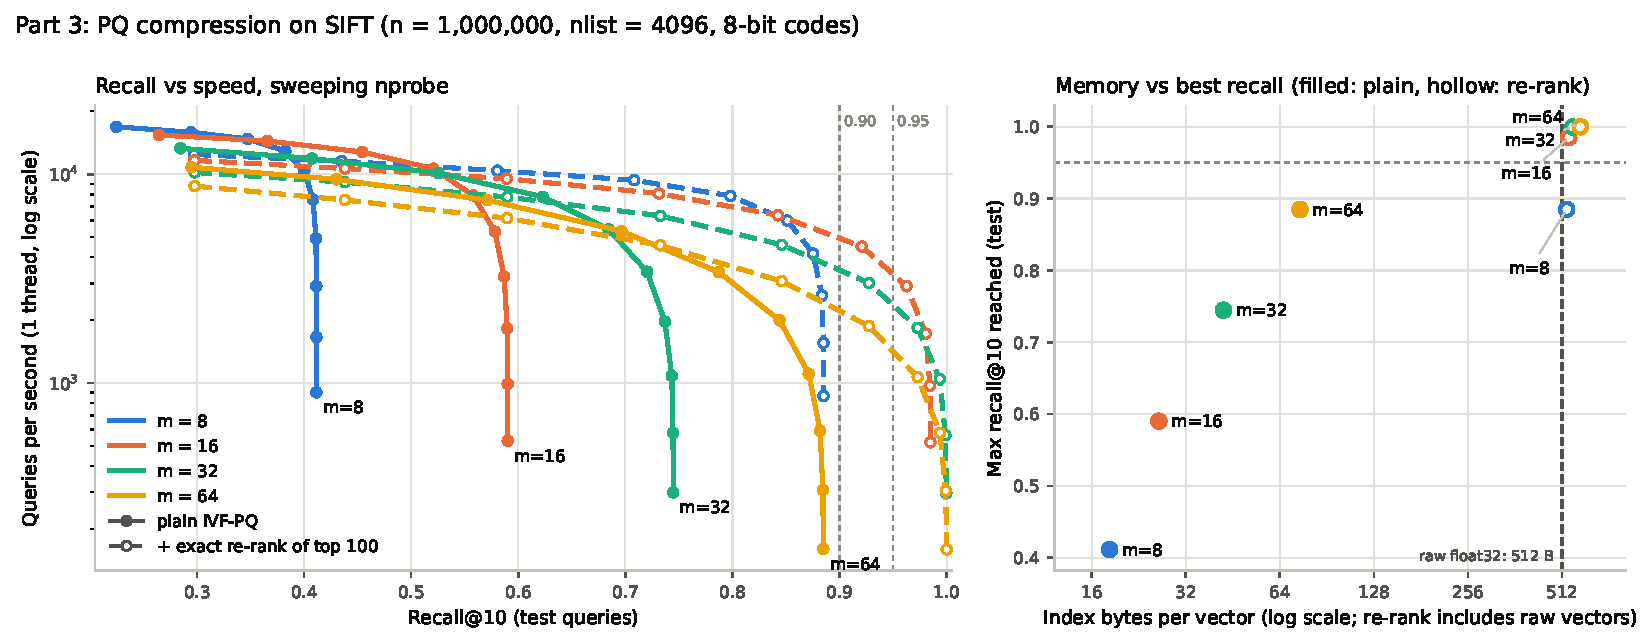
\includegraphics[width=\linewidth]{part3.pdf}
\caption{Part 3. Left: recall against QPS for each $m$ (solid: plain IVF-PQ; dashed: with exact
re-ranking of the top 100). Right: bytes per vector against the best recall reached.}
\label{fig:part3}
\end{figure}
\begin{table}[t]
\centering
\small
\begin{adjustbox}{max width=\linewidth}
\begin{tabular}{rlrrrrrr}
\toprule
m & Variant & Max recall@10 & QPS @0.90 (recall, nprobe) & QPS @0.95 (recall, nprobe) & Bytes/vector in RAM & PQ part bytes/vector & PQ code bytes \\
\midrule
8 & plain IVF-PQ & 0.412 & not reached & not reached & 18.3 & 18.3 & 8 \\
8 & IVF-PQ + re-rank top 100 & 0.885 & not reached & not reached & 530.3 & 18.3 & 8 \\
16 & plain IVF-PQ & 0.590 & not reached & not reached & 26.3 & 26.3 & 16 \\
16 & IVF-PQ + re-rank top 100 & 0.985 & 4,508 (0.921, nprobe=32) & 2,917 (0.963, nprobe=64) & 538.3 & 26.3 & 16 \\
32 & plain IVF-PQ & 0.745 & not reached & not reached & 42.3 & 42.3 & 32 \\
32 & IVF-PQ + re-rank top 100 & 1.000 & 3,014 (0.927, nprobe=32) & 1,841 (0.973, nprobe=64) & 554.3 & 42.3 & 32 \\
64 & plain IVF-PQ & 0.885 & not reached & not reached & 74.3 & 74.3 & 64 \\
64 & IVF-PQ + re-rank top 100 & 1.000 & 1,875 (0.927, nprobe=32) & 1,067 (0.973, nprobe=64) & 586.3 & 74.3 & 64 \\
\bottomrule
\end{tabular}
\end{adjustbox}
\caption{PQ compression on SIFT (nlist 4096, 8-bit codes): plain IVF-PQ vs the same index with exact re-ranking of the top 100 candidates. Single-thread QPS on the test queries (median of 3 runs). Max recall: test recall of the config with the highest tune recall. Configs are chosen on the tune queries (recall $\geq$ target); test recall is reported as measured and may fall slightly below the target. 'Bytes/vector in RAM' for re-rank includes the raw float32 vectors; 'PQ part' is the IVF-PQ index alone.}
\label{tab:part3}
\end{table}


\textbf{Results.}
\begin{itemize}
\item \emph{Plain IVF-PQ} has a recall ceiling that rises with $m$: 0.412, 0.590, 0.745 and 0.885
  for $m=8,16,32,64$. None reaches 0.90.
\item \emph{Re-ranking} raises the best recall to 0.885, 0.985, 1.000 and 1.000. For $m\ge16$ it
  reaches 0.95, at 2,917\,QPS for $m{=}16$ (nprobe 64) down to 1,067\,QPS for $m{=}64$.
\item \emph{Speed cost:} at the same nprobe, re-ranking costs a factor of 1.09 to 1.29 in QPS
  (median by $m$), and at most 1.42.
\item \emph{Memory:} plain IVF-PQ takes 18.3 to 74.3 bytes per vector. Re-ranking needs the raw
  float32 vectors in RAM, so it takes 530.3 to 586.3 bytes per vector, against 512 for the raw
  vectors alone.
\end{itemize}
Re-ranking buys back recall but gives up almost all of PQ's memory saving, unless the raw
vectors are read from disk, which we did not test.
% SOURCE: results/tables/part3.tex, results/part3_notes.md

%======================================================================
\clearpage
\section{Part 4: Drifting data (own data)}

\textbf{What changed.} We built a seeded generator from real SIFT vectors.
\begin{itemize}
\item The index is built on base vectors 0--200K.
\item Vectors 200K--400K are then added, moved by $s\cdot R\cdot u$. Here $u$ is a fixed
  random unit direction (seed 42) and $R=383.2$ is the mean distance of the base vectors to their
  centroid.
\item 2,000 queries (1,000 tune, 1,000 test) get the same shift.
\item Only the shift changes: $s\in\{0.25,0.5,1.0\}$, plus the control $s=0$. That is 400K
  vectors in total.
\item Each setting is compared \emph{stale} (trained or built on the base, then extended) against
  \emph{rebuilt} (built on all 400K). The indexes are IVF-Flat (nlist 1024) and HNSW ($M{=}32$),
  both swept as in Part 2. Ground truth is recomputed for every shift.
\end{itemize}
% SOURCE: config.py (PART4, SEED), results/results.csv (part=4, extra.R), annbench/synth.py

\begin{figure}[h]
\centering
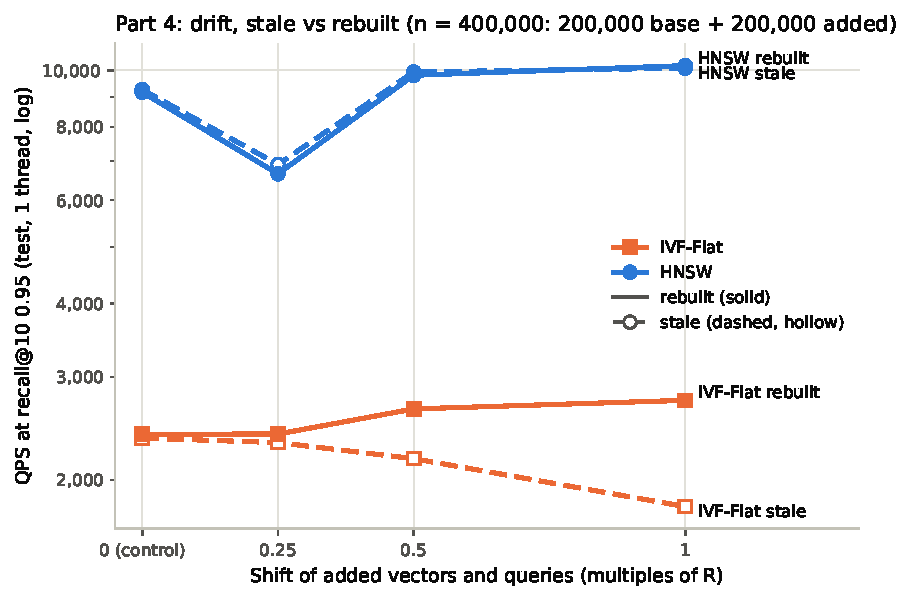
\includegraphics[width=0.62\linewidth]{part4.pdf}
\caption{QPS at recall 0.95 (test queries) against the shift of the added vectors and queries.
Solid: rebuilt; dashed, hollow: stale (extended after building).}
\label{fig:part4}
\end{figure}
\begin{table}[t]
\centering
\small
\begin{adjustbox}{max width=\linewidth}
\begin{tabular}{rllrrlrp{2.8cm}p{2.4cm}}
\toprule
Shift & Index & Variant & QPS @0.95 & Test recall & Setting & Dist. comps / query & IVF lists: CV / max$\div$mean / added in top 1\% & Time s \\
\midrule
0 & IVF-Flat & stale & 2,357 & 0.966 & nprobe=32 & 14,087 & 0.44 / 3.1 / 3\% & build 1.4, insert 0.3 \\
0 & IVF-Flat & rebuilt & 2,393 & 0.968 & nprobe=32 & 14,013 & 0.43 / 4.0 / 2\% & build 1.9 \\
0 & HNSW & stale & 9,272 & 0.952 & efSearch=32 & 985 & - & build 7.1, insert 10.8 \\
0 & HNSW & rebuilt & 9,176 & 0.951 & efSearch=32 & 986 & - & build 19.2 \\
0.25 & IVF-Flat & stale & 2,315 & 0.959 & nprobe=32 & 14,542 & 0.47 / 3.5 / 3\% & build 1.6, insert 0.3 \\
0.25 & IVF-Flat & rebuilt & 2,394 & 0.962 & nprobe=32 & 13,947 & 0.40 / 3.2 / 2\% & build 1.9 \\
0.25 & HNSW & stale & 6,907 & 0.971 & efSearch=48 & 1,289 & - & build 7.2, insert 10.7 \\
0.25 & HNSW & rebuilt & 6,657 & 0.975 & efSearch=48 & 1,337 & - & build 19.9 \\
0.5 & IVF-Flat & stale & 2,173 & 0.954 & nprobe=32 & 15,467 & 0.54 / 4.8 / 4\% & build 1.6, insert 0.3 \\
0.5 & IVF-Flat & rebuilt & 2,642 & 0.975 & nprobe=32 & 12,997 & 0.41 / 3.3 / 2\% & build 1.9 \\
0.5 & HNSW & stale & 9,935 & 0.953 & efSearch=32 & 931 & - & build 7.2, insert 8.6 \\
0.5 & HNSW & rebuilt & 9,808 & 0.954 & efSearch=32 & 939 & - & build 17.8 \\
1 & IVF-Flat & stale & 1,800 & 0.965 & nprobe=32 & 18,842 & 0.76 / 8.6 / 9\% & build 1.6, insert 0.3 \\
1 & IVF-Flat & rebuilt & 2,734 & 0.979 & nprobe=32 & 12,693 & 0.41 / 3.3 / 1\% & build 1.9 \\
1 & HNSW & stale & 10,085 & 0.956 & efSearch=32 & 914 & - & build 7.2, insert 7.3 \\
1 & HNSW & rebuilt & 10,187 & 0.954 & efSearch=32 & 914 & - & build 16.9 \\
\bottomrule
\end{tabular}
\end{adjustbox}
\caption{Drift experiment: 200,000 SIFT base vectors plus 200,000 added vectors and the queries shifted by shift $\times$ R along a fixed random direction. Stale = trained/built on the base, then extended; rebuilt = built on base + added. Single-thread QPS on the test queries at the config chosen on the tune queries for recall $\geq$ 0.95 (test recall reported as measured; 'not reached': highest-recall config shown). Distance computations per query exclude the IVF coarse quantizer (nlist per query).}
\label{tab:part4}
\end{table}


\textbf{What happened.}
\begin{itemize}
\item \emph{Stale IVF-Flat slows down as the shift grows.} From $s=0$ to $s=1$:
  \begin{itemize}
  \item the coefficient of variation of its list sizes rises from 0.44 to 0.76;
  \item the longest list grows from 3.1 to 8.6 times the mean;
  \item the share of added vectors in the largest 1\% of lists rises from 3\% to 9\%;
  \item distance computations per query rise from 14,087 to 18,842.
  \end{itemize}
  Rebuilt IVF-Flat needs 12,693 at $s=1$. So at $s=1$, stale IVF-Flat reaches 0.95 at 1,800\,QPS
  against 2,734 for rebuilt (ratio 0.66), while recall stays above 0.95.
\item \emph{HNSW is unaffected.} Stale and rebuilt HNSW stay within a QPS ratio of 0.99 to 1.04
  at every shift, with recall within 0.004. Adding the shifted vectors to a stale HNSW took 7.3 to
  10.8\,s, against 16.9 to 19.9\,s to rebuild from scratch.
\item \emph{The dip at $s=0.25$ is not drift.} HNSW at $s=0.25$ is slower for \emph{both}
  variants, because they needed efSearch 48 instead of 32 to reach 0.95 on the tune queries. It
  is a step of the sweep grid.
\end{itemize}
% SOURCE: results/tables/part4.tex, results/part4_notes.md

\textbf{Mechanism.} IVF's k-means centroids are frozen at training time. Shifted vectors are
assigned to the few cells whose centroids are nearest the new region, and those lists grow
long. The shifted queries probe exactly those lists, so each probe scans more vectors and QPS
falls. Retraining moves centroids into the new region and balances the lists again. HNSW has
nothing trained: each inserted vector links to its nearest neighbours at insertion time, so the
graph adapts to the new region.

\textbf{Hypothesis.}
\begin{itemize}
\item \emph{Supported:}
  \begin{itemize}
  \item the control behaves the same stale and rebuilt (0.98 for IVF, 1.01 for HNSW);
  \item IVF list imbalance grows with the shift, and the damage is to speed, not recall;
  \item rebuilding restores IVF speed (rebuilt QPS is 1.00 to 1.14 times the control);
  \item HNSW is robust.
  \end{itemize}
\item \emph{Not supported:} I predicted at least a 2$\times$ IVF slowdown at $s=1$; it was
  1.5$\times$.
\end{itemize}
\textbf{Not tested:} rotations, deletions, new clusters, IVF-PQ, shifts larger than $1.0R$, other
nlist and $M$, and queries from the old distribution after drift.
% SOURCE: results/part4_notes.md, hypothesis.md

\clearpage
%======================================================================
\section{Answers to the questions}

\subsection*{Q1. Fastest index at recall 0.95, and does it change between datasets?}
HNSW is the fastest on both datasets: 4,775 vs 1,697\,QPS for IVF-Flat on SIFT, and 518 vs
303\,QPS on GloVe. IVF-PQ cannot reach 0.95 at all. The winner does not change, but the costs do.
On GloVe, HNSW needs a larger graph ($M{=}32$) and a much wider search (efSearch 384 vs 64), and
both indexes are much slower than on SIFT at the same recall (HNSW 518 vs 4,775\,QPS;
IVF-Flat 303 vs 1,697\,QPS).

\emph{Why HNSW wins.} A greedy graph walk computes few distances, because each step moves to a
neighbour that is closer to the query. IVF must scan whole inverted lists, even though most of
the vectors in them are far from the query. On the 400K SIFT vectors of Part 4, at recall 0.95,
HNSW computed 914 to 1,337 distances per query, against 12,693 to 18,842 for IVF-Flat.

\emph{Why GloVe is harder.} The likely reason (we did not measure it) is that GloVe's word vectors
have weaker neighbourhood structure: a query's true neighbours are barely closer than many other
vectors, and they are spread over many IVF cells and graph regions. Both indexes must therefore
examine more candidates; IVF-Flat on GloVe needs nprobe 512 of 4096 lists.
% SOURCE: results/tables/part2_qps.tex, results/tables/part4.tex (distance computations per query)

\subsection*{Q2. Build time and memory; what PQ saves and gives up}
\begin{itemize}
\item \emph{Build time} (20 threads): HNSW took 60.8\,s on SIFT and 149.2\,s on GloVe; IVF-Flat
  took 18.9\,s and 18.1\,s; IVF-PQ took 62.3\,s and 35.4\,s.
\item \emph{Where the time goes:} HNSW pays at insertion, because every vector runs a search
  with efConstruction 200 to find its links. IVF pays mainly for k-means training: 13.5\,s of
  IVF-Flat's 18.9\,s on SIFT, and 51.7\,s of IVF-PQ's 62.3\,s, which adds PQ codebook training.
\item \emph{Memory:} HNSW stores the raw vectors plus about $2M$ neighbour ids per vector, so it
  needs 656.3 and 672.2 bytes per vector, against 512 and 400 for the raw vectors. IVF-Flat is
  the raw vectors plus an 8-byte id: 522.1 and 409.4.
\item \emph{What PQ saves:} it stores a code of $m$ bytes, 18.3 to 74.3 bytes per vector on SIFT.
\item \emph{What PQ gives up:} accuracy. Plain IVF-PQ tops out at 0.885 (SIFT) and 0.863 (GloVe).
  Getting recall back by re-ranking needs the raw vectors again (538.3\,B per vector for $m{=}16$
  at 2,917\,QPS), so the saving only survives if the exact vectors can live on disk.
\end{itemize}
% SOURCE: results/tables/part2_cost.tex, results/tables/part3.tex

\subsection*{Q3. What Parts 3 and 4 showed, and when headline numbers mislead}

\emph{Part 3 against my hypothesis.} These held:
\begin{itemize}
\item plain IVF-PQ is capped, and the cap rises with $m$ ($m{=}8$: 0.412, below my 0.60;
  $m{=}16$: 0.590, below 0.90);
\item re-ranking reaches 0.95 for $m\ge16$, while $m{=}8$ falls short (0.885), as I allowed;
\item re-ranking costs less than 2$\times$ in QPS (at most 1.42);
\item the memory estimates held: 18.3 to 74.3 bytes per vector measured, against 16 to 72
  predicted.
\end{itemize}
Two predictions were wrong:
\begin{itemize}
\item I said $m{=}64$ ``may come close to 0.95''. It stopped at 0.885.
\item I said larger $m$ costs only a ``slight'' QPS loss. At recall 0.95 with re-ranking, QPS
  fell from 2,917 ($m{=}16$) to 1,067 ($m{=}64$).
\end{itemize}

\emph{Part 4.} The control, the direction of the IVF damage, recovery by rebuilding and HNSW's
robustness all held. The size of the effect did not: the stale IVF slowdown at $s=1$ was
1.5$\times$, not the 2$\times$ I predicted.

\emph{When headline numbers mislead.}
\begin{itemize}
\item A ``bytes per vector'' headline for PQ is misleading unless it comes with the recall it
  reaches: the compact index cannot reach 0.95, and the index that can is no longer compact.
\item Headline QPS is measured on indexes built from the data they serve. Under drift, an IVF
  index that is extended rather than retrained serves slower than any number in Part 2 suggests,
  while HNSW does not.
\end{itemize}
% SOURCE: hypothesis.md, results/part3_notes.md (P4 predicted vs measured), results/tables/part3.tex, results/part4_notes.md

\begin{table}[t]
\centering
\small
\begin{adjustbox}{max width=\linewidth}
\begin{tabular}{lrrllllllp{4.5cm}}
\toprule
Dataset & n & Exact ms/query & Exact $\leq$ 100 ms & Raw GiB & HNSW GiB & IVF-Flat GiB & IVF-PQ GiB & IVF-PQ + re-rank GiB & Recommendation \\
\midrule
sift & 150,000 & 4.5 [M] & yes & 0.07 (fits) & 0.09 (fits) & 0.07 (fits) & 0.01 (fits) & 0.08 (fits) & Exact (IndexFlatL2): 4.5 ms/query, recall 1.0, 0.07 GiB; ANN not needed for the budget \\
sift & 10,000,000 & 324.9 [P] & no & 4.77 (fits) & 6.11 (fits) & 4.86 (fits) & 0.69 (fits) & 5.01 (fits) & HNSW: M=16, efSearch=64; 0.24 ms/query (extrapolated (x log n ratio; optimistic)); 6.1 GiB \\
glove & 150,000 & 3.3 [M] & yes & 0.06 (fits) & 0.09 (fits) & 0.06 (fits) & 0.01 (fits) & 0.06 (fits) & Exact (IndexFlatL2): 3.3 ms/query, recall 1.0, 0.06 GiB; ANN not needed for the budget \\
glove & 10,000,000 & 245.8 [P] & no & 3.73 (fits) & 6.26 (fits) & 3.81 (fits) & 0.54 (fits) & 4.27 (fits) & HNSW: M=32, efSearch=384; 2.22 ms/query (extrapolated (x log n ratio; optimistic)); 6.3 GiB \\
\bottomrule
\end{tabular}
\end{adjustbox}
\caption{Question 4: exact single-thread latency ([M] measured, [P] projected linearly in n from the measured full-size latency) and index memory (measured bytes/vector at the recall-0.95 config x n; IVF-PQ: highest-recall config, which does not reach 0.95; GloVe re-rank: plain IVF-PQ + raw vectors, not measured). 'fits' = at most 12 GiB, 'tight' = up to 16 GiB, 'no' = more. Recommendation rule: exact if it meets 100 ms and fits; otherwise the fastest recall-0.95 operating point that meets both (10M latencies are extrapolated). Single-thread, one query at a time.}
\label{tab:q4}
\end{table}


\subsection*{Q4. 150,000 or 10 million vectors, 100\,ms per query, 16\,GB RAM}

\emph{150,000 vectors: no ANN is needed.}
\begin{itemize}
\item Measured exact search takes 4.5\,ms per query on SIFT and 3.3\,ms on GloVe, with recall 1.0
  and 0.07 and 0.06\,GiB of raw vectors.
\item The linear model from the 1M timings predicted 4.87 and 3.69\,ms, so latency scales about
  linearly with $n$.
\item ANN would only be worth it if throughput mattered more than latency.
\end{itemize}

\emph{10 million vectors: use HNSW.}
\begin{itemize}
\item Exact search is \emph{projected} at 324.9\,ms (SIFT) and 245.8\,ms (GloVe) per query on one
  thread, well over budget, because every query scans all vectors.
\item HNSW at the measured 0.95 settings ($M{=}16$, efSearch 64 for SIFT; $M{=}32$, efSearch 384
  for GloVe) is \emph{extrapolated} to 0.24 and 2.22\,ms. Its graph search grows roughly with
  $\log n$, not $n$.
\item It needs 6.1 and 6.3\,GiB, inside 16\,GB, and every index fits.
\end{itemize}

\emph{Caveats at 10M.}
\begin{itemize}
\item Building needs the raw vectors and the graph in RAM at once (about 10.9 and 10.0\,GiB).
\item Build time extrapolates to about 12 and 24 minutes, optimistically.
\item efSearch would have to rise at 10M to keep recall at 0.95, which is not measured.
\item If memory became tight, IVF-PQ with re-ranking from disk would be the fallback.
\end{itemize}
% SOURCE: results/tables/q4.tex, results/q4_notes.md

\subsection*{Q5. Ways this benchmark could mislead}
\begin{enumerate}
\item \textbf{Machine-state drift (tested, not corrected).}
  \begin{itemize}
  \item During the overnight Part 2 run, the canary's QPS varied by 21.3\% on SIFT and 23.3\% on
    GloVe across sweeps.
  \item The quick pipeline took 9\,min 02\,s plugged in but 16\,min 52\,s on battery.
  \item Comparing two configs timed hours apart can be off by about this much.
  \item Pinning to one performance core and taking medians reduce noise within a measurement,
    not between measurements. Part 4's control (stale/rebuilt within 2\%) shows that close-in-time
    comparisons are much tighter.
  \end{itemize}
\item \textbf{``Batch'' speed depends on a library heuristic (tested).}
  \begin{itemize}
  \item FAISS 1.14.3 uses BLAS for a batch only when queries $\times$ dimension $\ge$ 128,000.
  \item In quick mode, 1,000 GloVe queries ($\times100$) fall below that, and the batch was only
    1.4$\times$ faster than one at a time, against 7.7$\times$ for SIFT.
  \item The Part 1 contrast is therefore a property of the query count and the library version,
    not only of the hardware. Our full runs use 5,000 queries, above the threshold.
  \end{itemize}
\item \textbf{Single thread, one query at a time, one machine (not tested elsewhere).}
  \begin{itemize}
  \item Servers batch queries and use many threads.
  \item In Part 1, 20 threads helped SIFT batch search (761 vs 342\,QPS) much more than GloVe
    (383 vs 348).
  \item The ranking of the indexes under multi-threaded serving, or on another CPU, was not
    measured.
  \end{itemize}
\item \textbf{Tune/test split (tested).}
  \begin{itemize}
  \item Configs are chosen on tune queries, so the test recall can land below the target.
  \item The gap between tune and test recall at the same config has a median of 0.0147 (SIFT)
    and 0.0043 (GloVe), and at most 0.0500.
  \item GloVe HNSW $M{=}16$ at efSearch 1024 shows the effect: test recall 0.9527 but tune recall
    0.9490, so it is not counted as reaching 0.95.
  \end{itemize}
\item \textbf{Tie tolerance (partly tested).}
  \begin{itemize}
  \item 65 of 10,000 SIFT queries have exact ties at the 10th neighbour. A tie-blind recall would
    score our exact search at 0.9935 set agreement instead of 1.0000.
  \item Tie handling is unit-tested, but we did not test how sensitive the results are to the
    value of $\epsilon$.
  \end{itemize}
\end{enumerate}
% SOURCE: results/part2_notes.md (canary, tune vs test), results_quick/run_times.txt (16 min 52 s,
% on battery: extra.power_plugged = false in results_quick/results.csv), logs/run_all_quick.log
% (9 min 02 s, plugged in), results/env.json (faiss_distance_compute_blas_threshold),
% results_quick/tables/part1.md (quick batch speed-ups), results/tables/part1.tex,
% results/results.csv (part=2, glove hnsw M=16 efSearch=1024), results/part1_agreement.json,
% results/tables/part4.tex

\end{document}
